\documentclass[10pt,c,aspectratio=1610,handout]{beamer}
\usetheme[block=fill,numbering=fraction,progressbar=frametitle]{metropolis}
%\usecolortheme{beaver}
\usepackage{textpos}
\usepackage{amsmath}
\usepackage{amssymb}
\usepackage{appendixnumberbeamer}

\setbeamercovered{transparent}

\newcommand\blfootnote[1]{%
  \begingroup
  \renewcommand\thefootnote{}\footnote{#1}%
  \addtocounter{footnote}{-1}%
  \endgroup
}

\renewcommand{\baselinestretch}{1.25}
% Colour theme
\definecolor{QDMblue}{rgb}{0.00, 0.1882, 0.3608}
\definecolor{QDMgold}{rgb}{0.9098, 0.6510, 0.0000}
\definecolor{QDMgreen}{rgb}{0.3098, 0.5490, 0.0510}
\setbeamercolor{normal text}{ fg= QDMblue , bg= white }
\setbeamercolor{alerted text}{ fg= QDMgold }
\setbeamercolor{example text}{ fg= QDMgreen }

\begin{document}

% Personal Info
\title{Lecture 07: A New-Keynesian Business Cycle Model}
\author[Konstantin Gantert]{\begin{large} Konstantin Gantert \end{large} \\ \textbf{Quantitative Dynamic Macroeconomics}}
\date{\textit{this version:} \today}

% Eliminates Navigation Bar on every Frame
\beamertemplatenavigationsymbolsempty

%-------------------------------------------------------------------------
% 0.1 Titlepage
%-------------------------------------------------------------------------
{\setbeamertemplate{footline}{} 
\frame{\titlepage}}
 \addtocounter{framenumber}{-1}
%-------------------------------------------------------------------------
% Outline for this Lecture
\begin{frame}{Outline for this Lecture}%
  \onslide<1->{%
    \begin{minipage}[c]{0.48\textwidth}%
      \textbf{What we have seen so far}%
      \begin{enumerate}%
        \item Stochastic CiA model with capital {\tiny [CG 1, 5]}%
        \item State-space and recursive methods {\tiny [CG 1, 5]}%
        \item Approximation \& undet. coeff. {\tiny [CG 3, 4]}%
        \item Calibration \& quantitative analysis {\tiny [CG 4, 5]}%
      \end{enumerate}%
    \end{minipage}%
  }%
  \hfill%
  \onslide<3->{%
    \begin{minipage}[c]{0.48\textwidth}%
      \textbf{What we will see today}%
      \begin{enumerate}%
        \item Price Adjustment Costs {\tiny [CG 1, 4, 5]}%
        \item Natural Rate Hypothesis {\tiny [CG 5, 6]}%
        \item Simulations and Analysis {\tiny [CG 1, 6]}%
      \end{enumerate}%
    \end{minipage}%
  }%
  \vspace*{0.25in}%
  \onslide<2->{%
    \begin{block}{Big Picture of the Lecture:}%
      \begin{enumerate}%
        \item How to model persistent aggregate demand effects in our model economy?%
        \item What impact does monetary policy have on our model economy?%
      \end{enumerate}%
    \end{block}%
  }%
\end{frame}%
%-------------------------------------------------------------------------
% X. Motivation - The Impact of Nominal Variables on the Economy
%-------------------------------------------------------------------------
\section{Motivation for Sticky Prices\\{\small Money Non-Neutrality in the Short-Run}}%
% Motivation: Short-Comings of the CiA/RBC Model
%-------------------------------------------------------------------------
\begin{frame}{Motivation: Short-Comings of the CiA Model/RBC}%
  Our CiA/RBC model has dealt with many issues of earlier macroeconomic models, such as:
  \begin{small}%
    \begin{itemize}%
      \item[$\blacktriangleright$] Micro-foundations and dynamic modeling%
      \item[$\blacktriangleright$] Random processes and rational expectations%
      \item[$\blacktriangleright$] General equilibrium%
    \end{itemize}%
  \end{small}%
  \vspace*{0.15in}%
  \pause%
  Why do we need another model then? \textbf{Short-comings of the CiA/RBC model:}%
  \pause%
  \begin{small}%
    \begin{itemize}%
      \item[$\blacktriangleright$] \textbf{Predominant Productivity Shocks:} Traditional Keynesians see productivity change as a source of long-run growth, not of short-run cycles, which are attributed to demand fluctuations.%
      \item[$\blacktriangleright$] \textbf{Efficiency of Markets:} There is no role for stabilization policy in a frictionless model.\\Keynes saw recessions as episodes of inefficient use of resources.%
      \item[$\blacktriangleright$] \textbf{Money:} The CiA/RBC model has a limited role for money and nominal variables. Only money growth has a one-period effect on real variables. This implies a limited role for monetary policy.%
    \end{itemize}%
  \end{small}%
\end{frame}%
% Motivation: Evidence on Money Non-Neutrality
%-------------------------------------------------------------------------
\begin{frame}{Motivation: Evidence on Money Non-Neutrality}%
  \begin{figure}%
    \centering%
    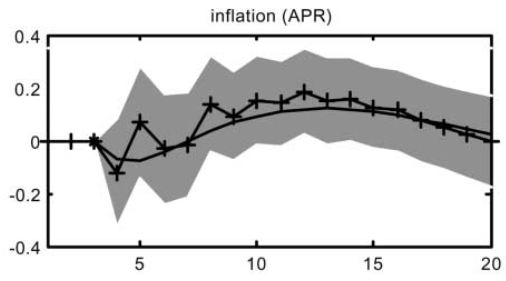
\includegraphics[width=0.45\textwidth]{figures/inflation_eM_christiano_2005.png}%
    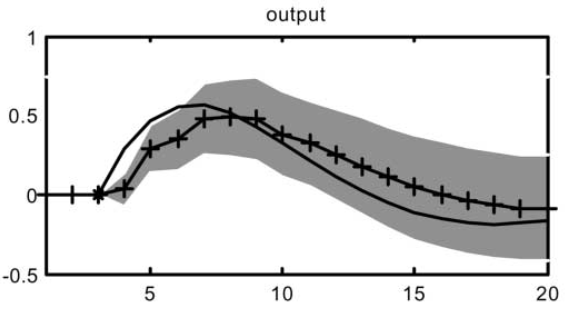
\includegraphics[width=0.45\textwidth]{figures/output_eM_christiano_2005.png}\\%
    {\scriptsize SOURCE: Christiano et al. (2005). NOTE: VAR-estimated IRFs to an expansionary monetary policy shock.}%
  \end{figure}%
  \begin{itemize}%
    \item[$\blacktriangleright$] \textbf{Money Non-Neutrality:} Real variables as output (also consumption, investment) increase following an expansionary monetary policy shock.%
    \item[$\blacktriangleright$] \textbf{Sticky Prices:} Inflation shows a hump-shaped behavior with high autocorrelation.%
  \end{itemize}%
\end{frame}%
% Ten Facts on Prices and their Implications for Macro Models (1/2)
%-------------------------------------------------------------------------
\begin{frame}{Ten Facts on Prices and their Implications for Macro Models (1/2)}%
  \begin{enumerate}%
    \item \textbf{Prices change at least once a year:}%
    \begin{itemize}%
      \item[$\rightarrow$] US CPI changes every 4 months, US PPI every 6-8 months, EU CPI is even stickier.%
    \end{itemize}%
    \vspace*{0.1in}%
    \pause%
    \item \textbf{Sales and product turnover are often important for micro price flexibility:}%
    \begin{itemize}%
      \item[$\rightarrow$] Micro price flexibility does not imply macro price flexibility.%
    \end{itemize}%
    \vspace*{0.1in}%
    \pause%
    \item \textbf{Reference prices are stickier and more persistent than regular prices:}%
    \begin{itemize}%
      \item[$\rightarrow$] Reference pricing behavior may suggest some form of sticky plan and/or sticky information.%
    \end{itemize}%
    \vspace*{0.1in}%
    \pause%
    \item \textbf{There is substantial heterogeneity in the frequency of price change across goods:}%
    \begin{itemize}%
      \item[$\rightarrow$] Service prices are stickier than those of goods. Among goods, ''raw'' goods (energy, fresh produce) are more flexible than ''processed'' goods.% 
    \end{itemize}%
    \vspace*{0.1in}%
    \pause%
    \item \textbf{More cyclical goods change prices more frequently:}%
    \begin{itemize}%
      \item[$\rightarrow$] Prices change more frequently in categories with more procyclical real consumption growth.%
    \end{itemize}%
  \end{enumerate}%
\end{frame}%
% Ten Facts on Prices and their Implications for Macro Models (2/2)
%-------------------------------------------------------------------------
\begin{frame}{Ten Facts on Prices and their Implications for Macro Models (2/2)}%
  \begin{enumerate}%
    \setcounter{enumi}{5}%
    \item \textbf{Price changes are big on average, but many small changes occur:}%
    \begin{itemize}%
      \item[$\rightarrow$] Many prices changes are larger than needed to keep up. However, many very small prices changes happen too. There is a ''missing middle''.%
    \end{itemize}%
    \vspace*{0.1in}%
    \pause%
    \item \textbf{Relative price changes are transitory:}%
    \begin{itemize}%
      \item[$\rightarrow$] Relative price movements tend to fade over time - they are less persistent than random walk.%
    \end{itemize}%
    \vspace*{0.1in}%
    \pause%
    \item \textbf{Price changes are typically not synchronized over the business cycle:}%
    \begin{itemize}%
      \item[$\rightarrow$] Periods of greater macro volatility may exhibit more synchronization.%
    \end{itemize}%
    \vspace*{0.1in}%
    \pause%
    \item \textbf{Neither frequency nor size is increasing in the age of a price:}%
    \begin{itemize}%
      \item[$\rightarrow$] Hazard rate of price changes is falling over the first few months and largely flat afterward.%
    \end{itemize}%
    \vspace*{0.1in}%
    \pause%
    \item \textbf{Price changes are linked to wage changes:}%
    \begin{itemize}%
      \item[$\rightarrow$] Firms with a higher share of labor costs in total make less frequent price adjustments, potentially resulting from the fact that wages adjust less frequently than other input prices.%
    \end{itemize}%
  \end{enumerate}%
  {\scriptsize See Klenow and Malin (2010) for a full analysis of prices.}%
\end{frame}%
% What are common ways of modeling sticky prices in the literature?
%-------------------------------------------------------------------------
\begin{frame}{What are common ways of modeling sticky prices in the literature?}%
  \begin{itemize}%
    \item[$\blacktriangleright$] \textbf{Information problems:} Asymmetric information concerning the money supply, or household demand. The information might be unavailable, or it is available but too costly {\scriptsize (e.g. Mankiw and Reis, 2002)}.%
    \pause%
    \item[$\blacktriangleright$] \textbf{Non-Walrasian features:} Markets are determined by prices and a second component, e.g. search costs for trade opportunities, simultaneously {\scriptsize (e.g. Kiyotaki and Wright, 1989)}.%
    \pause%
    \item[$\blacktriangleright$] \textbf{Adjustment costs:} It is costly to change prices. There is a trade-off between additional demand and adjustment costs {\scriptsize (i.e. Rotemberg, 1982)}.%
    \pause%
    \item[$\blacktriangleright$] \textbf{Pricing rules:} Firms follow rules to change prices:%
    \begin{itemize}%
      \item State-dependent pricing: Adjust when prices are relatively far away from some pre-specified target price {\scriptsize (i.e. Caplin and Spulber, 1987)}.%
      \item Time-dependent pricing: Adjust after a pre-specified amount of periods. {\scriptsize (i.e. Fischer, 1977; Taylor, 1980; Calvo, 1983)}.%
    \end{itemize}%
  \end{itemize}%
\end{frame}%
%-------------------------------------------------------------------------
% X. Frictional Price Setting
%-------------------------------------------------------------------------
\section{Frictional Price Setting\\{\small Applying Rotemberg (1982) to our Model}}%
% Model Overview - Five Types of Agents in the Model Economy
%-------------------------------------------------------------------------
\begin{frame}{Model Overview - Five Types of Agents in the Model Economy}%
  \vspace*{0.1in}%
  \begin{enumerate}%
    \item \textbf{Representative household:}%
    \begin{itemize}%
      \item[$\rightarrow$] Buy consumption and investment goods.%
      \item[$\rightarrow$] Supply labor and capital to firms.%
      \item[$\rightarrow$] Holds bonds, money, and capital as financial assets.%
      \item[$\rightarrow$] Receives government revenues and firm profits lump-sum at the end of the period.%
    \end{itemize}%
    \vspace*{0.1in}%
    \pause%
    \item \textbf{Representative final good firm:}%
    \begin{itemize}%
      \item[$\rightarrow$] Aggregate many different intermediate goods to one final good.%
    \end{itemize}%
    \vspace*{0.1in}%
    \pause%
    \item \textbf{Intermediate good firms of many different types $i \in I$:}%
    \begin{itemize}%
      \item[$\rightarrow$] Employ labor and capital to produce intermediate goods.%
      \item[$\rightarrow$] Sets intermediate good prices, but price adjustment is costly (Rotemberg (1982)).%
    \end{itemize}%
    \vspace*{0.1in}%
    \pause%
    \item \textbf{The government (fiscal policy):}%
    \begin{itemize}%
      \item[$\rightarrow$] Taxes labor and capital income of households. Rebates it lump-sum.%
    \end{itemize}%
    \vspace*{0.1in}%
    \pause%
    \item \textbf{The central bank (monetary policy):}%
    \begin{itemize}%
      \item[$\rightarrow$] Sets the nominal interest rate.%
    \end{itemize}%
  \end{enumerate}%
\end{frame}%
% Differentiating Between Individual and Aggregate Variables
%-------------------------------------------------------------------------
\begin{frame}{Differentiating Between Individual and Aggregate Variables}%
  \begin{block}{Remember from the lecture on taxes}%
    Firms are separate entities and input factors are traded on competitive markets. Households and firms choose individual levels, while market rates are determined by aggregate levels of labor and capital.%
  \end{block}%
  \vspace*{0.15in}%
  \pause%
  \textbf{Underlying assumptions:}%
  \begin{itemize}%
    \begin{small}%
      \item[$\blacktriangleright$] $w$ and $r$ are the prices such that labor and capital markets clear.%
      \item[$\blacktriangleright$] Many households and firms: Nobody is large enough to have an impact on market prices.%
      \item[$\blacktriangleright$] Every firm uses labor and capital from many households.%
      \item[$\blacktriangleright$] Every household supplies labor and capital to many firms.
    \end{small}%
  \end{itemize}%
\end{frame}%
% Household Utility Maximization
%-------------------------------------------------------------------------
\begin{frame}{Household Utility Maximization}%
  The \emph{representative household} maximizes his utility by choosing%
  \begin{align*}%
    \max_{C_t, \, L_t, \, B_{t+1}, \, K_{t+1}} \mathbb{E}_t \sum_{t=1,2} \beta^{t-1} \left[ log\left(C_t\right) - \frac{\varphi}{1+\gamma} L_t^{1+\gamma} \right] + \mathbb{E}_t \beta^2 \mathbb{V}_H \left(B_3,K_3\right)%
  \end{align*}%
  subject to%
  \begin{align*}%
    \frac{M_t}{\nu} \; = & \; P_t C_t,\\%
    q_{t} B_{t+1} + M_{t+1} \; = & \; P_t \left[ \left(1-\tau_L\right)w_t L_t + \left(1-\tau_K\right)r_t K_t\right] + M_t + B_t + T_t + \Pi_t\\%
    & \;  - P_t C_t - P_t \left[ K_{t+1} - \left(1-\delta\right) K_t \right],\\%
    K_{t+1} \; = & \; \left(1-\delta\right) K_t + X_t.%
  \end{align*}%
  \vspace*{0.1in}%
  \pause%
  \begin{block}{Atomistic households}%
    \begin{small}%
      Household income depends on the market rates for labor, $(1-\tau_L) w_t$, and capital, $(1-\tau_K) r_t$. Like in the lecture on taxes, the labor and capital decisions of households do not affect their market rates.%
    \end{small}%
  \end{block}%
\end{frame}%
% Household First-Order Conditions
%-------------------------------------------------------------------------
\begin{frame}{Household First-Order Conditions}%
  Applying a change-in-variables, $\mu_t = \frac{\beta^{t-1}}{P_t C_t} \tilde{\mu_t}$, to render the model stationary, we are left with the \emph{usual household first-order conditions:}%
  \begin{align}%
    w_t \; = & \; \varphi L_t^\gamma \frac{C_t}{\left(1-\tau_L\right) \tilde{\mu}_t}\\%
    \notag\\%
    \tilde{\mu}_t \; = & \; \beta \mathbb{E}_t \frac{P_t}{P_{t+1}} \frac{C_t}{C_{t+1}} \frac{1}{\nu} \left[ 1 - \left(1-\nu\right) \tilde{\mu}_{t+1} \right]\\%
    \notag\\%
    q_t \; = & \; \beta \mathbb{E}_t \frac{P_t}{P_{t+1}} \frac{C_t}{C_{t+1}} \frac{\tilde{\mu}_{t+1}}{\tilde{\mu}_t}\\%
    \notag\\%
    1 \; = & \; \beta \mathbb{E}_t \left[ \left(1-\tau_K\right) r_{t+1} + \left(1-\delta\right) \right] \frac{C_t}{C_{t+1}} \frac{\tilde{\mu}_{t+1}}{\tilde{\mu}_t}%
  \end{align}%
\end{frame}%
% Final Good Firms as Goods Bundler
%-------------------------------------------------------------------------
\begin{frame}{Final Good Firms as Goods Bundler}%
  Final good firms maximize profits by bundling \emph{differentiated goods} to one good according to%
  \begin{align*}%
    \max_{Y_t,Y_t(i)} \; \left[ {P}_t Y_t - \int_0^1 P_t(i) Y_t(i) di \right]%
  \end{align*}%
  subject to household preferences%
  \begin{align*}%
    Y_t \; = \; \left[ \int_0^1 Y_t(i)^\rho di \right]^{\frac{1}{\rho}}%
  \end{align*}%
  which they take into account as they sell the final good to households later on.\\%
  \vspace*{0.15in}%
  \pause%
  \begin{block}{Optimal demand for good \textit{i} (first-order condition):}%
    \begin{align}%
      P_t(i) \; = \; \left[ \frac{Y_t}{Y_t(i)} \right]^{1-\rho} {P}_t%
    \end{align}%
    \vspace*{-0.2in}%
    \begin{small}%
      \begin{itemize}%
        \item[$\blacktriangleright$] If $P_t(i)>P_t$, demand is \textbf{not} zero. If $P_t(i)<P_t$, demand is \textbf{not} equal to $C_t$.%
        \item[$\blacktriangleright$] \textbf{Monopolistic Competition} {\footnotesize (Dixit \& Stiglitz, 1977)}:  Goods are imperfect substitutes (set by $\rho$)!%
      \end{itemize}%
    \end{small}%
  \end{block}
\end{frame}%
% Intermediate Good Firms: Production and Price Setting
%-------------------------------------------------------------------------
\begin{frame}{Intermediate Good Firms: Production and Price Setting}%
  An intermediate good firm of type \textit{i} maximizes its profits by choosing%
  \begin{align*}%
    \max_{Y_t(i), \, L_t(i), \, K_t(i), \, P_t(i)} \; \mathbb{E}_t \sum_{t=1,2} \beta^{t-1} \frac{\mu_t}{\mu_1} \left\{ P_t(i) Y_t(i) - W_t L_t(i) - {P}_t r_t K_t(i) \right\} + \mathbb{E}_t \beta^2 \frac{\mu_3}{\mu_1} \mathbb{V}_F \left(P_2, P_3\right)%
  \end{align*}%
  subject to%
  \begin{align*}%
    Y_t(i) \; = & \; \left[Z_t L_t(i)\right]^{1-\alpha} K_t(i)^\alpha \left[ 1 - \frac{\kappa}{2} \left( \frac{P_t(i)}{P_{t-1}(i)} - 1 \right)^2 \right],\\%
    P_t(i) \; = & \; \left[\frac{Y_t}{Y_t(i)}\right]^{1-\rho} {P}_t,%
  \end{align*}%
  and where $\Gamma \left( P_t(i),P_{t-1}(i) \right) = \frac{\kappa}{2} \left( \frac{P_t(i)}{P_{t-1}(i)} - 1 \right)^2$.\\%
  \pause%
  \vspace*{0.1in}%
  \begin{small}%
    \textbf{Properties of the firm:}%
    \begin{itemize}%
      \item[$\blacktriangleright$] It anticipates the demand function of the final good firm.%
      \pause%
      \item[$\blacktriangleright$] It maximizes its profits by \textbf{setting prices} under quadratic price adjustment costs, $\Gamma_t$.%
      \item[$\blacktriangleright$] Firms are owned by households, hence they discount the future the same way, $\beta^{t-1} \frac{\mu_t}{\mu_1}$.%
    \end{itemize}%
  \end{small}%
  \vspace*{-0.2in}%
\end{frame}%
% Intermediate Good Firms: First-Order Conditions
%-------------------------------------------------------------------------
\begin{frame}{Intermediate Good Firms: First-Order Conditions}%
  \textbf{Input factor demand functions:}%
  \begin{align}%
    w_t \; = & \; \left(1-\alpha\right) \frac{Y_t(i)}{L_t(i)} mc_t(i)\\%
    r_{t} \; = & \; \alpha \frac{Y_{t}(i)}{K_{t}(i)} mc_{t}(i)%
  \end{align}%
  \pause%
  \begin{block}{Price setting condition:}%
    \begin{align}%
      \begin{split}%
        \frac{\kappa \left(\frac{P_{t}(i)}{P_{t-1}(i)}-1\right) \frac{P_t(i)}{P_{t-1}(i)}}{1-\frac{\kappa}{2}\left(\frac{P_{t}(i)}{P_{t-1}(i)}-1\right)^2} \; = & \; \frac{1-\frac{\rho}{mc_t(i)}}{1-\rho}\\%
        & \; + \mathbb{E}_t q_t \frac{\kappa \left(\frac{P_{t+1}(i)}{P_t(i)}-1\right) \frac{P_{t+1}(i)}{P_t(i)}}{1-\frac{\kappa}{2}\left(\frac{P_{t+1}(i)}{P_t(i)}-1\right)^2} \frac{P_{t+1}(i)}{P_t(i)} \frac{Y_{t+1}(i)}{Y_t(i)} \frac{mc_{t+1}(i)}{mc_t(i)}%
      \end{split}%
    \end{align}%
    \vspace*{-0.15in}%
    \begin{small}%
      \begin{itemize}%
        \item[$\blacktriangleright$] \textbf{Steady-state:} Price markup, $\mathcal{M} = \frac{1}{mc} = \frac{1}{\rho}$, that depends on elasticity of substitution, $\rho$.%
        \item[$\blacktriangleright$] \textbf{Dynamics:} Markup fluctuates over the business cycle due to sticky prices.%
      \end{itemize}%
    \end{small}%
  \end{block}%  
\end{frame}%
% General Equilibrium
%-------------------------------------------------------------------------
\begin{frame}{General Equilibrium}%
  \textbf{Representative agents:}%
  \begin{itemize}%
    \begin{small}%
      \item[$\blacktriangleright$] All households have symmetric preferences and characteristics.%
      \item[$\blacktriangleright$] All intermediate firms have the same technologies.%
    \end{small}%
  \end{itemize}%
  \vspace*{0.15in}%
  \pause%
  \textbf{Equilibrium - all markets clear:}%
  \begin{itemize}%
    \begin{small}%
      \item[$\blacktriangleright$] Good markets clear, $C_t + X_t = Y_t = \int_0^1 Y_t(i) di$.%
      \item[$\blacktriangleright$] Labor markets clear, $L^D_t = L^S_t$ (this pins down $w_t$).%
      \item[$\blacktriangleright$] Capital rental markets clear, $K^D_t = K^S_t$ (this pins down $r_t$).%
      \item[$\blacktriangleright$] Money markets clear, $M_t = \bar{M}_t$.%
      \item[$\blacktriangleright$] The nominal bond price, $q_t$, adjusts such that bonds are in zero supply, $B_t = 0$.%
    \end{small}%
  \end{itemize}%
  \vspace*{0.15in}%
  \pause%
  \textbf{Assumptions about tax and profit distribution:}%
  \begin{itemize}%
    \begin{small}%
      \item[$\blacktriangleright$] Government revenues are rebated to the households lump-sum, $\tau_L w_t L_t + \tau_K r_t K_t = T_t$.%
      \item[$\blacktriangleright$] Firm profits, $\Pi_t$, are redistributed to all households equally.%
    \end{small}%
  \end{itemize}%
\end{frame}%
% Summary of the Model in Symmetric Equilibrium
%-------------------------------------------------------------------------
\begin{frame}{Summary of the Model in Symmetric Equilibrium}%
  \begin{small}%
    \vspace*{-0.2in}%
    \begin{align}%
      \text{Labor market:} \quad & \varphi L_t^\gamma \frac{C_t}{(1-\tau_L) \tilde{\mu}_t} \; = \; \left(1-\alpha\right) \frac{Y_t}{L_t} mc_t\\%
      \text{Capital market:} \quad & \tilde{\mu}_t \; = \; \beta \mathbb{E}_t \left[ \left(1-\tau_K\right) \alpha \frac{Y_{t+1}}{K_{t+1}} mc_{t+1} + \left(1-\delta\right) \right] \frac{C_t}{C_{t+1}} \tilde{\mu}_{t+1}\\%
      \text{Bond market:} \quad & q_t \; = \; \beta \mathbb{E}_t \frac{1}{1+\pi_{t+1}} \frac{C_t}{C_{t+1}} \frac{\tilde{\mu}_{t+1}}{\tilde{\mu}_t}\\%
      \text{Money demand:} \quad & \tilde{\mu}_t \; = \; \beta \mathbb{E}_t \frac{1}{1+\pi_{t+1}} \frac{C_t}{C_{t+1}} \frac{1}{\nu} \left[ 1 - \left(1-\nu\right) \tilde{\mu}_{t+1} \right]\\%
      \text{Phillips curve:} \quad & \Omega\left(\pi_t\right) \; = \; \frac{1-\frac{\rho}{mc_t}}{1-\rho} + \mathbb{E}_t q_t \left(1+\pi_{t+1}\right) \frac{Y_{t+1}}{Y_t} \frac{mc_{t+1}}{mc_t} \Omega\left(\pi_{t+1}\right)\\%
      \text{Resource constraint:} \quad & C_t \; = \; Y_t - K_{t+1} + (1-\delta) K_t\\%
      \text{Production function:} \quad & Y_t \; = \; \left[Z_t L_t\right]^{1-\alpha} K_t^\alpha%
    \end{align}%
    \vspace*{-0.4in}%
    \begin{itemize}
      \item[$\rightarrow$] We use $\frac{{P}_{t+1}}{{P}_t} = 1 + \pi_{t+1}$ for the inflation rate and $\Omega(\pi) \equiv \frac{\kappa \pi (1+\pi)}{1-\frac{\kappa}{2}\pi^2}$ for the marginal price adjustment cost.%
      \item[$\rightarrow$] We have $8$ endogenous variables ($C_t, L_t, K_t, Y_t, \tilde{\mu}_t, mc_t, \pi_t, q_t$), but only $7$ equilibrium equations: \textbf{Indeterminacy!}%
      \item[$\rightarrow$] We need a \textbf{Taylor rule} for $q_t = 1/(1+r_{B,t})$. Money supply is not exogenous: it adjusts to implement the targeted rate, $1+\tau_t = \mathbb{E}_t(1+\pi_{t+1})C_{t+1}/C_t$!%
    \end{itemize}
  \end{small}%
  \vspace{-0.2in}%
\end{frame}%
%-------------------------------------------------------------------------
% Monetary Policy and the Natural Interest Rate
%-------------------------------------------------------------------------
\section{Monetary Policy\\and the Natural Interest Rate}%
% Setting the Nominal Interest Rate
%-------------------------------------------------------------------------
\begin{frame}{Setting the Nominal Interest Rate}%
  \begin{block}{Central Bank Policy according to Taylor (1993, 1999):}%
    \begin{align}%
      \frac{1+r_{B,t}}{1+\bar{r}_{B}} \; = & \; \left(\frac{1+\pi_t}{1+\bar{\pi}}\right)^{\theta_\pi} \times \left( 1+Y_{Gap,t} \right)^{\theta_{Gap}} \times exp(M_t)%
    \end{align}%
    \vspace*{-0.2in}%
    \begin{itemize}%
      \item[$\rightarrow$] Estimated equation that represents interest rate setting behavior of modern central banks!%
    \end{itemize}%
  \end{block}%
  \pause%
  \begin{itemize}%
    \item[$\blacktriangleright$] \textbf{Policy Coefficients:} $\theta_\pi,\theta_{Gap} \geq 0$. Determine the reaction function of monetary policy.%
    \begin{itemize}%
      \item[$\rightarrow$] \textbf{Taylor principle:} To ensure determinacy of the economy, we must set $\theta_\pi>1$ (credible threat). Otherwise, there are sunspot equilibria!%
    \end{itemize}%
    \pause%
    \item[$\blacktriangleright$] \textbf{Target Shock:} $M_t \in \mathbb{R}$. Summarizes deviations from (expected) monetary policy.%
    \pause%
    \item[$\blacktriangleright$] \textbf{Interest Rate Target:} $\bar{r}_B \in \mathbb{R}$. Target steady-state nominal interest rate.\\%
  \end{itemize}%
  \vspace*{0.1in}%
  \begin{center}%
    \begin{large}%
      What determines $\bar{r}_B$ and $Y_{Gap,t}$?%
    \end{large}%
  \end{center}%
\end{frame}%
% Determining the Optimal Nominal Interest Rate Target
%-------------------------------------------------------------------------
\begin{frame}{Determining the Optimal Nominal Interest Rate Target}%
  The \textbf{steady-state nominal interest rate} is given by the bond Euler equation%
  \begin{align*}%
    1+\bar{r}_B \; = \; \frac{1+\bar{\pi}}{\beta} \left(1+g\right)%
  \end{align*}%
  \pause%
  Equivalently, the \textbf{natural interest rate} (social planner) is given by%
  \begin{align*}%
    1+r_B^* \; = \; \frac{1}{\beta} \left(1+g\right)%
  \end{align*}%
  \pause%
  Therefore, the \textbf{long-run stable intertemporal output allocation} is given by a Fisher equation%
  \begin{align*}%
    1+\bar{r}_B \; = \; \left(1+r_B^*\right) \left(1+\bar{\pi}\right),%
  \end{align*}%
  where%
  \begin{itemize}%
    \item[$\rightarrow$] $r_B^*$ determines the fundamental intertemporal features of the economy (social planner),%
    \item[$\rightarrow$] $\bar{\pi}$ is a target inflation rate (set by the central bank).%
  \end{itemize}%
  \vspace*{0.3in}%
  \begin{quotation}%
    What determines 1) the natural interest rate and 2) the target inflation rate?%
  \end{quotation}%
\end{frame}%
% Drivers of the Natural Interest Rate and Target Inflation
%-------------------------------------------------------------------------
\begin{frame}{Drivers of the Natural Interest Rate and Target Inflation}%
  Possible drivers of the \textbf{natural interest rate} in reality:%
  \begin{itemize}%
    \item[$\blacktriangleright$] \textbf{NK Model:} Household discount rate across time, $\frac{1}{\beta}-1$.%
    \item[$\blacktriangleright$] \textbf{OLG Models:} Demographics and the global savings glut.%
    \item[$\blacktriangleright$] \textbf{TFP Growth:} Slowdown in productivity growth, $g$.%
    \pause%
    \item[$\Rightarrow$] It becomes increasingly clear that \textbf{$r_B^*$ has decreased} over the last 30 years.\\{\scriptsize (Laubach \& Williams (2003); Holston, Laubach \& Williams (2017))}.%
    \item[$\Rightarrow$] This pushes $\bar{r}_B$ closer to the \textbf{zero lower bound}!%
  \end{itemize}%
  \vspace*{0.1in}%
  \pause%
  Possible drivers of the \textbf{target inflation rate} in reality:%
  \begin{itemize}%
    \item[$\blacktriangleright$] Allows asymmetric downward rigid prices and wages to adjust.%
    \item[$\blacktriangleright$] Creates head-space to prevent deflationary spirals.%
    \item[$\blacktriangleright$] (De-)anchoring of inflation expectations in periods of high inflation.%
  \end{itemize}%
\end{frame}%
% The U.S. Natural Interest Rate
%-------------------------------------------------------------------------
\begin{frame}{The U.S. Natural Interest Rate {\scriptsize (Laubach \& Williams, 2003)}}%
  \begin{figure}%
    \centering%
    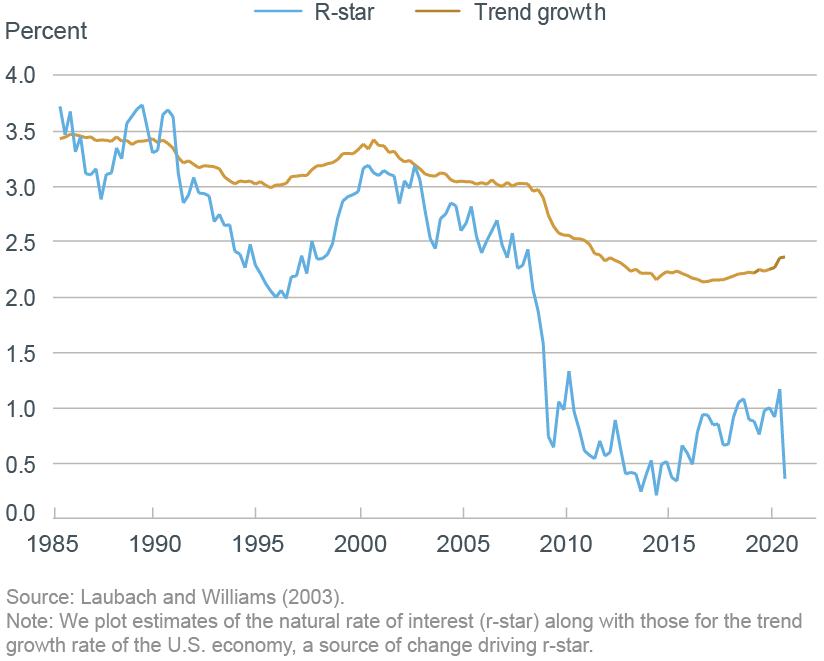
\includegraphics[width=0.75\linewidth]{figures/LW_nat_interest_rate.png}\\%
    {\scriptsize SOURCE: Based on the Laubach-Williams natural rate estimates of the Federal Reserve Bank of New York, \url{https://www.newyorkfed.org/research/policy/rstar}.}%
  \end{figure}%
\end{frame}%
% The Output Gap: Definition
%-------------------------------------------------------------------------
\begin{frame}%
  \frametitle{The Output Gap: Definition}%
  The output gap is given by:%
  \begin{align}%
    Y_{Gap,t} \; = & \; \frac{\tilde{Y}_t}{\tilde{Y}_{N,t}} - 1%
  \end{align}%
  \begin{itemize}%
    \item[$\blacktriangleright$] The output gap is defined as actual output relative to natural (potential) output.\vspace{0.1in}%
    \pause%
    \item[$\blacktriangleright$] The natural rate of the economy prevails \textbf{absent any frictions or imperfections} in the market economy. HERE: $\rho = 1$, and $\kappa = 0$. {\scriptsize (This economy is equivalent to the social planner solution.)}\vspace{0.1in}%
    \pause%
    \item[$\blacktriangleright$] Deviations from potential output, $\tilde{Y}_{N,t}$, follow from sticky prices over the business cycle.%
    \begin{itemize}%
      \footnotesize%
      \item[$\rightarrow$] Positive deviations indicate the economy being above its long-run potential.%
      \item[$\rightarrow$] Negative deviations indicate the economy being below its long-run potential.%
    \end{itemize}%
  \end{itemize}%
\end{frame}%
%-------------------------------------------------------------------------
% X. A Calibrated NK Model and the Data
%-------------------------------------------------------------------------
\section{A Calibrated NK Model\\and the Data}%
% Policy Functions, State Variables, and Exogenous Shocks
%-------------------------------------------------------------------------
\begin{frame}{Policy Functions, State Variables, and Exogenous Shocks}%
  \small%
  We solve the dynamic model by its \textbf{policy functions} (symmetric for natural rate model):\\%
  \begin{footnotesize}%
  \begin{minipage}{0.5\textwidth}%
    \begin{align*}%
      C_t \; = & \; \Lambda_C \left(K_t, Z_t, M_t\right)\\%
      L_t \; = & \; \Lambda_L \left(K_t, Z_t, M_t\right)\\%
      K_{t+1} \; = & \; \Lambda_K \left(K_t, Z_t, M_t\right)\\%
      Y_t \; = & \; \Lambda_Y \left(K_t, Z_t, M_t\right)%
    \end{align*}%
  \end{minipage}%
  \hfill%
  \begin{minipage}{0.5\textwidth}%
    \begin{align*}%
      \tilde{\mu}_t \; = & \; \Lambda_{\tilde{\mu}} \left(K_t, Z_t, M_t\right)\\%
      mc_t \; = & \; \Lambda_{mc} \left(K_t, Z_t, M_t\right)\\%
      \pi_t \; = & \; \Lambda_{\pi} \left(K_t, Z_t, M_t\right)\\%
      r_{B,t} \; = & \; \Lambda_r \left(K_t, Z_t, M_t\right)%
    \end{align*}%
  \end{minipage}\\%
  \end{footnotesize}%
  \vspace*{0.2in}%
  \pause%
  \textbf{Forward-looking variables:}%
  \begin{itemize}%
    \item[$\blacktriangleright$] $\mathbb{E}_t C_{t+1}$: Intertemporal consumption allocation by the Euler equation!%
    \item[$\blacktriangleright$] $\mathbb{E}_t \pi_{t+1}$: Intertemporal pricing by the Phillips curve!
    \item[$\blacktriangleright$] $\mathbb{E}_t \tilde{\mu}_{t+1}$: Intertemporal asset allocation by the capital Euler equation!%
  \end{itemize}%
  \pause%
  \textbf{Exogenous Shock Processes:}%
    \begin{align*}%
      Z_t \; = & \; \rho_Z Z_{t-1} + \varepsilon_{Z,t}, \quad \varepsilon_{Z,t} \sim \mathcal{N} \left(0,\sigma_{Z,t}^2\right)\\%
      M_t \; = & \; \rho_M M_{t-1} + \varepsilon_{M,t}, \quad \varepsilon_{M,t} \sim \mathcal{N} \left(0,\sigma_{M,t}^2\right)%
    \end{align*}%
  \pause%
  \vspace*{-0.2in}%
  \begin{itemize}%
    \item[$\Rightarrow$] We ask Dynare to do all those calculations for us!%
  \end{itemize}%
\end{frame}%
% Calibrating our Model Economy
%-------------------------------------------------------------------------
\begin{frame}{Calibrating our Model Economy}%
  \begin{table}%
    \centering%
    \footnotesize%
    \renewcommand{\arraystretch}{0.9}%
    \begin{tabular}{l c| l c}%
      \hline%
      Variable & Value & Variable & Value\\%
      \hline \hline%
      $\beta$ & $0.98$ & $\sigma_Z$ & $0.01$\\%
      $\sigma$ & $1$ & $\sigma_M$ & $0.005$\\%
      $\gamma$ & $\frac{1}{0.72}$ & $\sigma_P$ & $0.05$\\%
      $\nu$ & $0.5$ & $\rho_Z$ & $0.9$ \\%
      $\delta$ & $0.025$ & $\rho_M$ & $0.5$ \\%
      $\alpha$ & $0.33$ & $\rho_P$ & $0.5$ \\%
      $\rho$ & $0.9$ & $\theta_\pi$ & $1.5$ \\%
      $\kappa$ & $60$ & $\phi_X$ & $4$\\%
      \hline%
    \end{tabular}%
    \caption{Calibration overview}%
  \end{table}%
  \pause%
  \small%
  \begin{itemize}%
    \item[$\blacktriangleright$] Zero inflation steady state ($\pi^* = 0$), no taxes ($\tau_L = \tau_K = 0$), $\theta_R = \theta_Y = 0$ in the Taylor rule.%
    \item[$\blacktriangleright$] There is no exogenous growth of productivity or money supply in this model!%
    \pause%
    \item[$\blacktriangleright$] $\beta=0.98$ implies $8.4 \%$ nominal interest per year.%
    \item[$\blacktriangleright$] $\rho=0.9$ implies average price markups of $11 \%$.%
    \item[$\blacktriangleright$] $\alpha=\frac{1}{3}$ implies roughly one-third capital income share (markups distort it a bit).%
  \end{itemize}%
\end{frame}%
% Impulse Response Functions for a Model with Marginal Capital
%-------------------------------------------------------------------------
\begin{frame}{Impulse Response Functions for a Model with Marginal Capital}%
  We assume here: $\alpha \approx 0$ and $\delta = 1$!\\%
  \vspace*{0.15in}%
  \begin{minipage}{0.58\textwidth}%
    \begin{figure}%
    \centering%
    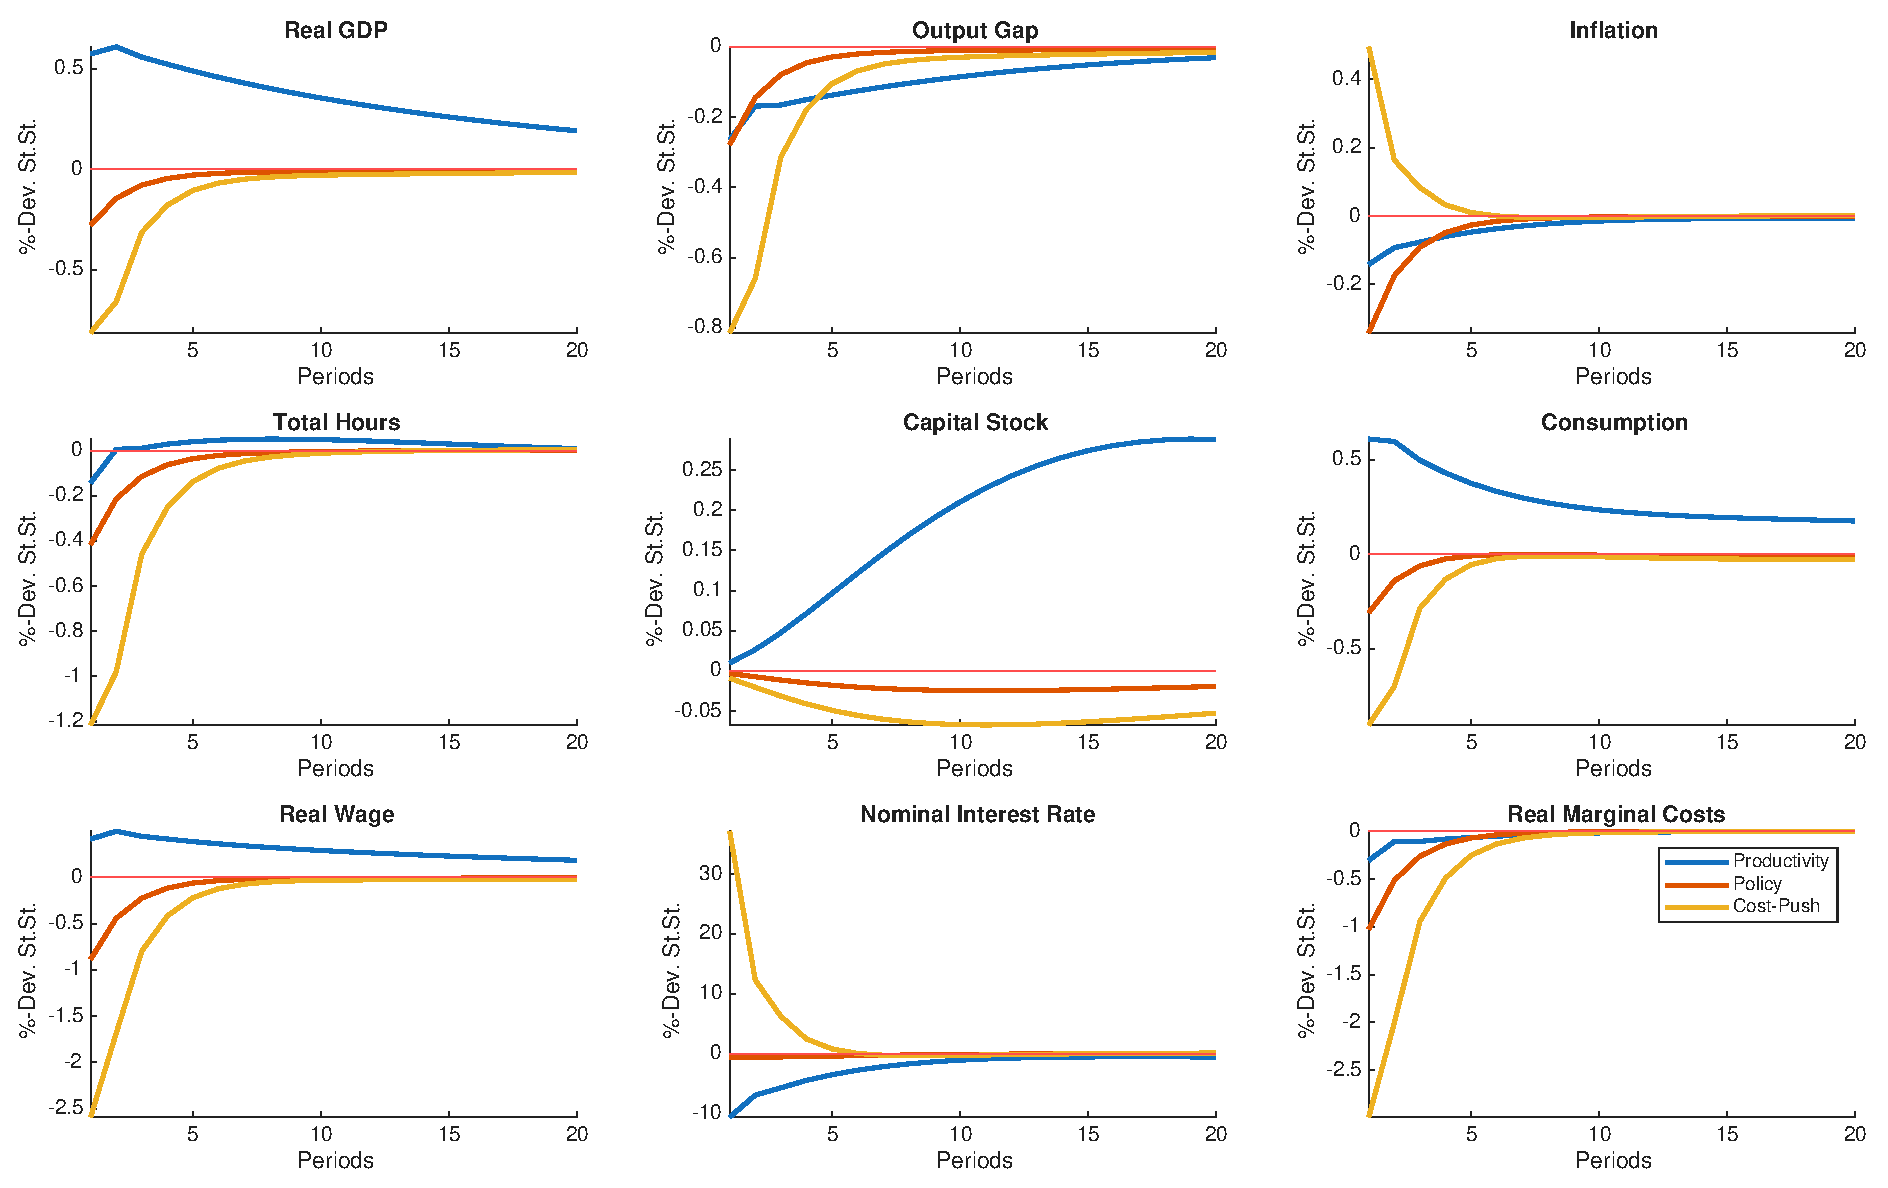
\includegraphics[width=\textwidth]{figures/irfs_without_capital.eps}%
  \end{figure}%
  \end{minipage}%
  \hfill%
  \pause%
  \begin{minipage}{0.4\textwidth}%
    \small%
    An increase in productivity, $Z_t$, leads to:%
    \begin{footnotesize}%
    \begin{itemize}%
      \item[$\blacktriangleright$] $mc_t \downarrow \; \Rightarrow \; \pi_t \downarrow \; \Rightarrow \; Y_t, C_t, K_t \uparrow$%
      \item[$\blacktriangleright$] $\pi_t \downarrow \; \Rightarrow \; r_{B,t} \downarrow$%
      \item[$\blacktriangleright$] $\pi_t \downarrow \text{ (but sticky!) } \; \Rightarrow \; Y_{Gap,t} \downarrow$%
      \item[$\blacktriangleright$] $w_t \uparrow \text{, but sticky } \pi_t \downarrow \; \Rightarrow \; L_t \downarrow$%
    \end{itemize}%
    \end{footnotesize}%
    \vspace*{0.1in}%
    \pause%
    A rise in interest rates, $r_{B,t}$, leads to:%
    \begin{footnotesize}%
      \begin{itemize}%
        \item[$\blacktriangleright$] $C_t \downarrow \; \Rightarrow \; Y_t, K_t, L_t \downarrow$%
        \item[$\blacktriangleright$] $Y_t \downarrow \; \Rightarrow \; mc_t, \pi_t \downarrow$%
        \item[$\blacktriangleright$] $\pi_t \downarrow \text{(but sticky!)} \; \Rightarrow \; Y_{Gap,t}, w_t \downarrow$%
      \end{itemize}%
    \end{footnotesize}%
  \end{minipage}%
\end{frame}%
% Impulse Response Functions for a Model with Capital
%-------------------------------------------------------------------------
\begin{frame}{Impulse Response Functions for a Model with Capital}%
  We assume here: $\alpha = \frac{1}{3}$ and $\delta = 0.03$! Hence, $K_t$ becomes a state variable!\\%
  \vspace*{0.15in}%
  \begin{minipage}{0.58\textwidth}%
    \begin{figure}%
    \centering%
    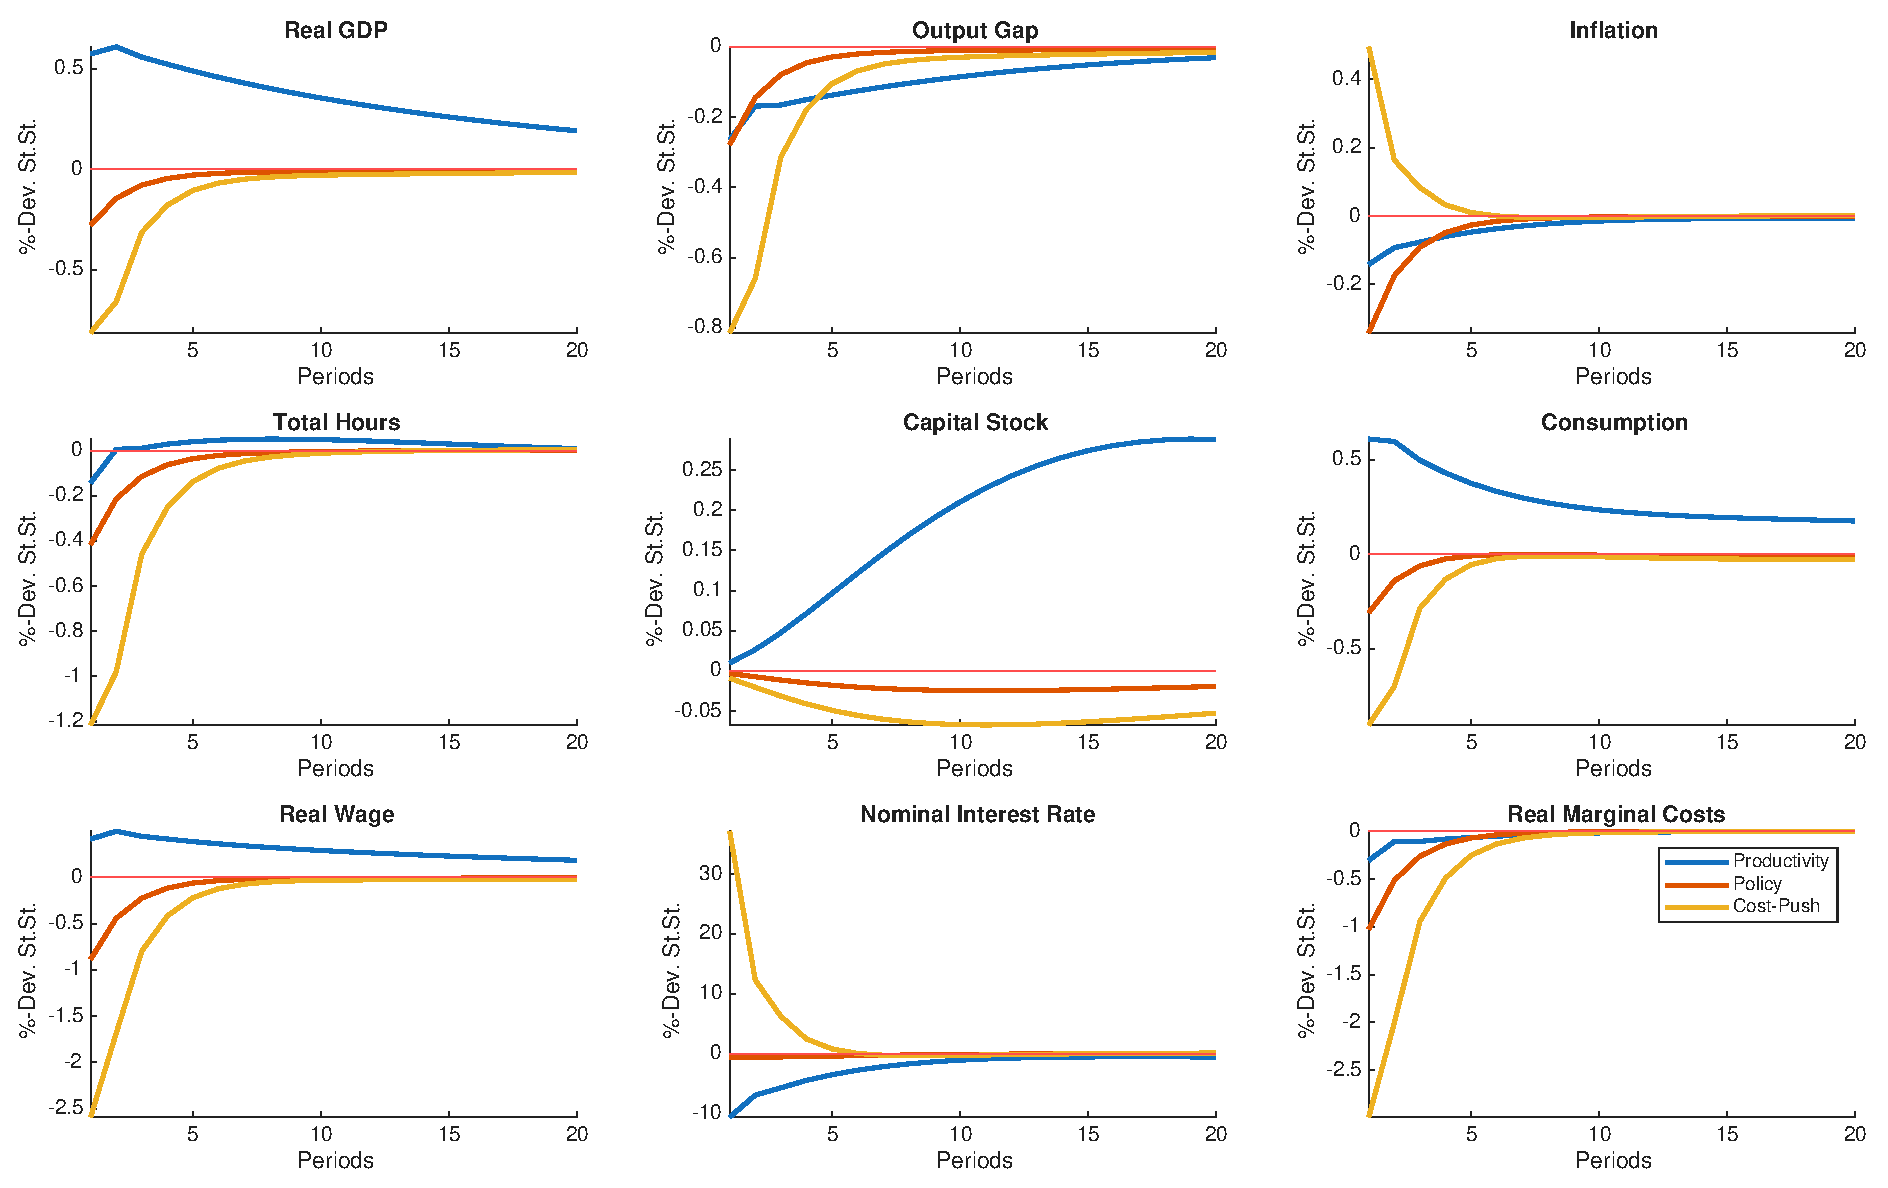
\includegraphics[width=\textwidth]{figures/irfs_with_capital.eps}%
  \end{figure}%
  \end{minipage}%
  \hfill%
  \pause%
  \begin{minipage}{0.4\textwidth}%
    \small%
    An increase in productivity, $Z_t$, leads to:%
    \begin{footnotesize}%
    \begin{itemize}%
      \item[$\blacktriangleright$] $Y_t, K_t, C_t \uparrow$ as before!%
      \item[$\blacktriangleright$] $Z_t \uparrow$ saved for later through $K_t \uparrow \uparrow$%
      \item[$\blacktriangleright$] It follows $Y_t \uparrow \uparrow \; \Rightarrow \; mc_t, \pi_t, L_t, Y_{Gap,t} \uparrow$%
      \item[$\blacktriangleright$] $\pi_t \uparrow \; \Rightarrow \; r_{B,t} \uparrow$%
      \item[$\blacktriangleright$] Higher persistence b/c $\delta < 1$%
    \end{itemize}%
    \end{footnotesize}%
    \vspace*{0.1in}%
    \pause%
    A rise in interest rates, $r_{B,t}$, leads to:%
    \begin{footnotesize}%
      \begin{itemize}%
        \item[$\blacktriangleright$] Mostly symmetric to case w/o capital.%
        \item[$\blacktriangleright$] Higher persistence through $\delta < 1$.%
        \item[$\blacktriangleright$] $Y_t, \pi_t \downarrow \downarrow \; \Rightarrow \; r_{B,t} \downarrow$!%
      \end{itemize}%
    \end{footnotesize}%
  \end{minipage}%
\end{frame}%
%-------------------------------------------------------------------------
% X. Conclusion
%-------------------------------------------------------------------------
\section{Conclusion}%
%-------------------------------------------------------------------------
% Summarizing the Lecture
\begin{frame}{Summarizing the Lecture}%
  \begin{center}%
    \begin{large}%
      Can you summarize the three main aspects of the lecture?%
    \end{large}%
  \end{center}%
\end{frame}%
% Conclusion
%-------------------------------------------------------------------------
\begin{frame}{Conclusion}%
  \begin{block}{Big Picture of the Lecture:}%
    \begin{enumerate}%
      \item How to model persistent aggregate demand effects in our model economy?%
      \item What impact does monetary policy have on our model economy?%
    \end{enumerate}%
  \end{block}%
  \pause%
  The \textbf{New Keynesian Model} allows for persistent aggregate demand effects:%
  \begin{itemize}%
    \item[$\blacktriangleright$] \textbf{Monopolistic competition:} Firms are price setters and charge a price markup.%
    \item[$\blacktriangleright$] \textbf{Sticky prices:} There is a trade-off between optimal prices and adjustment costs!%
  \end{itemize}%
  \pause%
  A \textbf{cyclical output gap} indicates a sub-optimal short-run equilibrium:%
  \begin{itemize}%
    \item[$\blacktriangleright$] Sticky prices prevent instantaneous price adjustment leading to distorted input allocation.%
  \end{itemize}%
  \pause%
  \textbf{Monetary policy} can control the nominal interest rate:%
  \begin{itemize}%
    \item[$\blacktriangleright$] It has real (persistent) effects as prices are sticky.%
    \item[$\blacktriangleright$] Inflation targeting can stabilize the economy.%
  \end{itemize}%
  \pause%
  \textbf{New Neoclassical Synthesis:} Prices are sticky in the short-run, but flexible in the long-run!{\scriptsize{} (Textbook treatments: Gal\'i, 2015; Cole, 2020)}%
\end{frame}%
% REFERENCES AND APPENDIX
%-------------------------------------------------------------------------
\begin{frame}{References (1/2)}%
  \begin{scriptsize}%
    \begin{itemize}%
      \item[$\blacktriangleright$] Calvo, G. A. (1983). Staggered prices in a utility-maximizing framework. Journal of Monetary Economics, 12(3), 383-398.%
      \item[$\blacktriangleright$] Caplin, A. S., \& Spulber, D. F. (1987). Menu costs and the neutrality of money. The Quarterly Journal of Economics, 102(4), 703-725.%
      \item[$\blacktriangleright$] Christiano, L. J., Eichenbaum, M., \& Evans, C. L. (2005). Nominal rigidities and the dynamic effects of a shock to monetary policy. Journal of Political Economy, 113(1), 1-45.%
      \item[$\blacktriangleright$] Cole, Harold L. (2020). Monetary and Fiscal Policy through a DSGE Lens. Oxford University Press.%
      \item[$\blacktriangleright$] Dixit, A. K., \& Stiglitz, J. E. (1977). Monopolistic competition and optimum product diversity. The American Economic Review, 67(3), 297-308.%
      \item[$\blacktriangleright$] Fischer, S. (1977). Long-term contracts, rational expectations, and the optimal money supply rule. Journal of Political Economy, 85(1), 191-205.%
      \item[$\blacktriangleright$] Gal\'i, J. (2015). Monetary Policy, Inflation, and the Business Cycle: An Introduction to the New Keynesian Framework and Its Applications. Princeton University Press.%
      \item[$\blacktriangleright$] Holston, K., Laubach, T., \& Williams, J. C. (2017). Measuring the natural rate of interest: International trends and determinants. Journal of International Economics, 108, 59-75.%
    \end{itemize}%
  \end{scriptsize}%
\end{frame}%
%-------------------------------------------------------------------------
\begin{frame}{References (2/2)}%
  \begin{scriptsize}%
    \begin{itemize}%
      \item[$\blacktriangleright$] Kiyotaki, N., \& Wright, R. (1989). On money as a medium of exchange. Journal of Political Economy, 97(4), 927-954.%
      \item[$\blacktriangleright$] Klenow, P. J., \& Malin, B. A. (2010). Microeconomic evidence on price-setting. In Handbook of Monetary Economics (Vol. 3, pp. 231-284). Elsevier.%
      \item[$\blacktriangleright$] Laubach, T., \& Williams, J. C. (2003). Measuring the natural rate of interest. Review of Economics and Statistics, 85(4), 1063-1070.%
      \item[$\blacktriangleright$] Mankiw, N. G., \& Reis, R. (2002). Sticky information versus sticky prices: A proposal to replace the New Keynesian Phillips curve. The Quarterly Journal of Economics, 117(4), 1295-1328.%
      \item[$\blacktriangleright$] Rotemberg, J. J. (1982). Monopolistic price adjustment and aggregate output. The Review of Economic Studies, 49(4), 517-531.%
      \item[$\blacktriangleright$] Taylor, J. B. (1980). Aggregate dynamics and staggered contracts. Journal of Political Economy, 88(1), 1-23.%
      \item[$\blacktriangleright$] Taylor, J. B. (1993). Discretion versus policy rules in practice. In Carnegie-Rochester Conference Series on Public Policy (Vol. 39, pp. 195-214). North-Holland.%
      \item[$\blacktriangleright$] Taylor, J. B. (1999). A historical analysis of monetary policy rules. In Monetary Policy Rules (pp. 319-348). University of Chicago Press.%
    \end{itemize}%
  \end{scriptsize}%
\end{frame}%
%-------------------------------------------------------------------------
\end{document}%